\documentclass[12pt]{article}
\usepackage{amsmath} %a widely used math package
\usepackage[
backend=biber,
style=phys,
sorting=none,
]{biblatex}
\addbibresource{refs.bib}%path to bib file

\usepackage{halloweenmath}
\usepackage{hyperref}
\hypersetup{
    colorlinks=true,
    linkcolor=blue!65!black,
	linkcolor=blue!65!black,
    filecolor=blue!65!black,    
    urlcolor=blue!65!black,
	citecolor=blue!65!black
    } 
\urlstyle{same}
\usepackage{enumitem} %for (a) (b) (c) enumeration
\usepackage{fullpage} %sets the margins to 1 inch. Turn off for the more restrictive TeX default
\usepackage{graphicx}
\usepackage{tkz-euclide}

%user-defined commands
\renewcommand{\vec}[1]{\mathbf{#1}} %Dr. Hamilton likes vectors denoted this way (boldface upright)
\newcommand{\gradient}{\boldsymbol{\nabla}}
\newcommand{\divergence}{\boldsymbol{\nabla}\cdot}
\newcommand{\curl}{\boldsymbol{\nabla}\times}
\newcommand{\Laplacian}{\nabla^2}

\usepackage{lipsum}
%fonts
\usepackage{newtx}
%\usepackage{kpfonts}

\title{My first \LaTeX \space document}
\author{Your Name}

\begin{document}
\maketitle

\section{This is the first section}
Here's in-line math: \(\partial p/\partial t\) is an acoustic jerk. Hey, so am I! \(\alpha, \beta\) for Greek letters. For displayed equations,
\begin{equation}
\vec{F} = m\vec{a}\,.
\end{equation}
For non-numbered equations, include the asterisk: 
\begin{equation*}
\vec{p} = m\vec{v}\,.
\end{equation*}
To refer to equations, use \texttt{label} with \texttt{eqref}:
\begin{equation}\label{eq:newton}
\vec{F} = m\vec{a}\,.
\end{equation}
Equation~\eqref{eq:newton} is Newton's law. The tilde prevents a line break. Dr.~Hamilton is smart; in this case, the tilde prevents a double space after the period. 

For aligned equations, use  
\begin{align*}
\vec{p} &= m\vec{v}\\
&= m\dot{\vec{x}}\,.
\end{align*}
Figure \ref{fig:ashby} looks good! Here's some filler text.
\lipsum
\begin{figure}%[h!]
\centering\includegraphics[width=0.5\linewidth]{fig/ashby}
\caption{Parameter space of acoustic metamaterials, where the density \(\rho\) is the horizontal axis and the compressibility \(\beta\) is the vertical axis. A similar parameter space could be drawn for electromagnetics (for which \(\rho\) and \(\beta\) would be replaced by \(\epsilon\) and \(\mu\)).} \label{fig:ashby}
\end{figure}

\lipsum

\section{This is the second section}

\begin{table}[h]
\centering\small
\begin{tabular}{ c | c c c c}
	$\ell$ & $\chi_n$ & $\chi_n^{1/2}$ & $\Delta_n = \chi^{1/2}_{n+1}-\chi^{1/2}_n$ & $\Delta_{n+1}-\Delta_{n}$\\\hline\hline
	1& 0.3564 & 0.5970 & 0.3500& $-0.0250$\\  
	2& 0.8966 & 0.9469 & 0.3250 & $-0.0045$\\  
	3& 1.6177 & 1.2719 & 0.3205 & 0.0033\\ 
	4& 2.5357 & 1.5924 & 0.3238 & 0.0058\\  
	5& 3.6718 & 1.9162 & 0.3296 & 0.0056\\  
	6& 5.0436 & 2.2458 & 0.3352 & 0.0044\\  
	7& 6.6614 & 2.5810 & 0.3395 & 0.0032\\  
	8& 8.5294 & 2.9205 & 0.3428 & 0.0023\\  
	9& 10.6489 & 3.2633& 0.3450 & 0.0016\\  
	10& 13.0196 & 3.6083 & 0.3466 & 0.0012\\  
	11& 15.6413 & 3.9549 & 0.3479 & 0.0009\\  
	12& 18.5138 & 4.3028 & 0.3488 & 0.0007\\  
	13& 21.6368 & 4.6515 & 0.3495 & 0.0006\\  
	14& 25.0102 & 5.0010 & 0.3500 & 0.0005\\  
	15& 28.6339 & 5.3511 & 0.3505 & 0.0004\\  
	16& 32.5078 & 5.7016 & 0.3509 & 0.0003\\  
	17& 36.6319 & 6.0524 & 0.3512 & 0.0002\\ 
	18& 41.0062 & 6.4036 & 0.3514 & 0.0002\\  
	19& 45.6305 & 6.7550 & 0.3517 & 0.0002\\   
	20& 50.5050 & 7.1067 & 0.3518 & 0.0002\\  
	21& 55.6295 & 7.4585 & 0.3520 & 0.0001\\   
	22& 61.0041 & 7.8105 & 0.3521 & 0.0001\\  
	23& 66.6288 & 8.1626 & 0.3523 &  \\
	24& 72.5035 & 8.5149 &  & \\\hline  
	50& 313.0008 & 17.6918 & 0.3533 & 0.0000 \\  
	51& 325.6258 & 18.0451 & 0.3533 & 0.0000 \\
	52& 338.5007 & 18.3984 & 0.3533 & 0.0000 \\  
	53& 351.6257 & 18.7517 & 0.3533 & 0.0000 \\
	54& 365.0007 & 19.1050 & 0.3533 & 0.0000 \\  
	55& 378.6257 & 19.4583 & 0.3533 & 0.0000 \\
	56& 392.5006 & 19.8116 & 0.3533 & 0.0000 \\  
	57& 406.6256 & 20.1650 & 0.3533 &\\
	58& 421.0006 & 20.5183 &  & \\\hline 
	70& 613.0004 & 24.7588 & 0.3534 & 0.0000 \\  
	71& 630.6254 & 25.1123 & 0.3534 & 0.0000 \\
	72& 648.5004 & 25.4657 & 0.3534 & 0.0000 \\  
	73& 666.6254 & 25.8191 & 0.3534 & \\
	74& 685.0004 & 26.1725 &  &\\
\end{tabular}
\caption{Tabulated values of the maximum of an equation for various values of $\ell$ ranging from \(1\) to \(74\). The fourth column shows how the difference $\Delta_n$ between subsequent values of $\chi_n^{1/2}$ generally grows as the orbital number increases, and the fifth column shows how the difference of the differences vanish as the orbital number decreases.}\label{table:parax:roots2}
\end{table}


\section*{Non-numbered section}

\begin{figure}
\begin{center}


\tikzset{every picture/.style={line width=0.75pt}} %set default line width to 0.75pt        

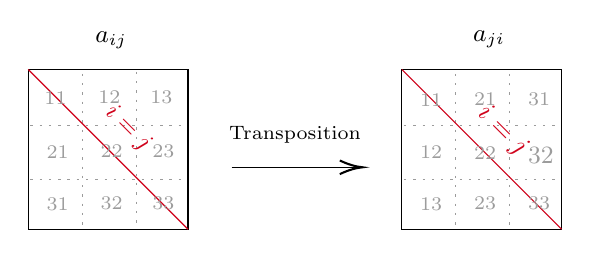
\begin{tikzpicture}[x=0.75pt,y=0.75pt,yscale=-1,xscale=1]
%uncomment if require: \path (0,99); %set diagram left start at 0, and has height of 99

%Straight Lines [id:da3686952917845694] 
\draw [color={rgb, 255:red, 155; green, 155; blue, 155 }  ,draw opacity=1 ] [dash pattern={on 0.84pt off 2.51pt}]  (231.47,20.4) -- (231.47,94.4) ;
%Straight Lines [id:da46454354486104354] 
\draw [color={rgb, 255:red, 155; green, 155; blue, 155 }  ,draw opacity=1 ] [dash pattern={on 0.84pt off 2.51pt}]  (257.47,19.42) -- (257.47,93.42) ;
%Straight Lines [id:da7610428286780471] 
\draw [color={rgb, 255:red, 155; green, 155; blue, 155 }  ,draw opacity=1 ] [dash pattern={on 0.84pt off 2.51pt}]  (206.47,45.4) -- (281.47,45.4) ;
%Straight Lines [id:da7271209617220877] 
\draw [color={rgb, 255:red, 155; green, 155; blue, 155 }  ,draw opacity=1 ] [dash pattern={on 0.84pt off 2.51pt}]  (206.47,71.4) -- (281.47,71.4) ;
%Straight Lines [id:da9458279316034213] 
\draw [color={rgb, 255:red, 155; green, 155; blue, 155 }  ,draw opacity=1 ] [dash pattern={on 0.84pt off 2.51pt}]  (386.47,71.4) -- (461.47,71.4) ;
%Straight Lines [id:da42476886331581865] 
\draw [color={rgb, 255:red, 155; green, 155; blue, 155 }  ,draw opacity=1 ] [dash pattern={on 0.84pt off 2.51pt}]  (386.47,45.4) -- (461.47,45.4) ;
%Straight Lines [id:da3084567265781819] 
\draw [color={rgb, 255:red, 155; green, 155; blue, 155 }  ,draw opacity=1 ] [dash pattern={on 0.84pt off 2.51pt}]  (411.47,20.4) -- (411.47,94.4) ;
%Straight Lines [id:da36884859012724514] 
\draw [color={rgb, 255:red, 155; green, 155; blue, 155 }  ,draw opacity=1 ] [dash pattern={on 0.84pt off 2.51pt}]  (437.47,20.4) -- (437.47,94.42) ;
%Shape: Rectangle [id:dp45286711431417515] 
\draw   (205.43,18.29) -- (282.43,18.29) -- (282.43,95.29) -- (205.43,95.29) -- cycle ;
%Straight Lines [id:da7039561565934498] 
\draw [color={rgb, 255:red, 208; green, 2; blue, 27 }  ,draw opacity=1 ][fill={rgb, 255:red, 155; green, 155; blue, 155 }  ,fill opacity=1 ]   (205.43,18.29) -- (282.43,95.29) ;
%Shape: Rectangle [id:dp9609288434207952] 
\draw   (385.43,18.29) -- (462.43,18.29) -- (462.43,95.29) -- (385.43,95.29) -- cycle ;
%Straight Lines [id:da16981815210379358] 
\draw [color={rgb, 255:red, 208; green, 2; blue, 27 }  ,draw opacity=1 ][fill={rgb, 255:red, 155; green, 155; blue, 155 }  ,fill opacity=1 ]   (385.43,18.29) -- (462.43,95.29) ;
%Straight Lines [id:da18376883328551608] 
\draw    (303.47,65.4) -- (364.47,65.4) ;
\draw [shift={(366.47,65.4)}, rotate = 180] [color={rgb, 255:red, 0; green, 0; blue, 0 }  ][line width=0.75]    (10.93,-3.29) .. controls (6.95,-1.4) and (3.31,-0.3) .. (0,0) .. controls (3.31,0.3) and (6.95,1.4) .. (10.93,3.29)   ;

% Text Node
\draw (247.85,32.16) node [anchor=north west][inner sep=0.75pt]  [font=\small,color={rgb, 255:red, 208; green, 2; blue, 27 }  ,opacity=1 ,rotate=-45]  {$i=j$};
% Text Node
\draw (212,27.88) node [anchor=north west][inner sep=0.75pt]  [font=\scriptsize]  {$\textcolor[rgb]{0.61,0.61,0.61}{11}$};
% Text Node
\draw (238,27.4) node [anchor=north west][inner sep=0.75pt]  [font=\scriptsize]  {$\textcolor[rgb]{0.61,0.61,0.61}{12}$};
% Text Node
\draw (263,27.4) node [anchor=north west][inner sep=0.75pt]  [font=\scriptsize]  {$\textcolor[rgb]{0.61,0.61,0.61}{13}$};
% Text Node
\draw (213,53.88) node [anchor=north west][inner sep=0.75pt]  [font=\scriptsize]  {$\textcolor[rgb]{0.61,0.61,0.61}{21}$};
% Text Node
\draw (239,53.4) node [anchor=north west][inner sep=0.75pt]  [font=\scriptsize]  {$\textcolor[rgb]{0.61,0.61,0.61}{22}$};
% Text Node
\draw (264,53.4) node [anchor=north west][inner sep=0.75pt]  [font=\scriptsize]  {$\textcolor[rgb]{0.61,0.61,0.61}{23}$};
% Text Node
\draw (213,78.82) node [anchor=north west][inner sep=0.75pt]  [font=\scriptsize]  {$\textcolor[rgb]{0.61,0.61,0.61}{31}$};
% Text Node
\draw (239,78.33) node [anchor=north west][inner sep=0.75pt]  [font=\scriptsize]  {$\textcolor[rgb]{0.61,0.61,0.61}{32}$};
% Text Node
\draw (264,78.33) node [anchor=north west][inner sep=0.75pt]  [font=\scriptsize]  {$\textcolor[rgb]{0.61,0.61,0.61}{33}$};
% Text Node
\draw (301,44.48) node [anchor=north west][inner sep=0.75pt]   [align=left] {{\scriptsize Transposition}};
% Text Node
\draw (427.85,32.16) node [anchor=north west][inner sep=0.75pt]  [color={rgb, 255:red, 208; green, 2; blue, 27 }  ,opacity=1 ,rotate=-45]  {$i=j$};
% Text Node
\draw (393,28.88) node [anchor=north west][inner sep=0.75pt]  [font=\scriptsize]  {$\textcolor[rgb]{0.61,0.61,0.61}{11}$};
% Text Node
\draw (419,28.4) node [anchor=north west][inner sep=0.75pt]  [font=\scriptsize]  {$\textcolor[rgb]{0.61,0.61,0.61}{21}$};
% Text Node
\draw (445,28.4) node [anchor=north west][inner sep=0.75pt]  [font=\scriptsize]  {$\textcolor[rgb]{0.61,0.61,0.61}{31}$};
% Text Node
\draw (393,53.88) node [anchor=north west][inner sep=0.75pt]  [font=\scriptsize]  {$\textcolor[rgb]{0.61,0.61,0.61}{12}$};
% Text Node
\draw (419,54.4) node [anchor=north west][inner sep=0.75pt]  [font=\scriptsize]  {$\textcolor[rgb]{0.61,0.61,0.61}{22}$};
% Text Node
\draw (445,54.4) node [anchor=north west][inner sep=0.75pt]  [font=\small]  {$\textcolor[rgb]{0.61,0.61,0.61}{32}$};
% Text Node
\draw (393,78.82) node [anchor=north west][inner sep=0.75pt]  [font=\scriptsize]  {$\textcolor[rgb]{0.61,0.61,0.61}{13}$};
% Text Node
\draw (419,78.33) node [anchor=north west][inner sep=0.75pt]  [font=\scriptsize]  {$\textcolor[rgb]{0.61,0.61,0.61}{23}$};
% Text Node
\draw (445,78.33) node [anchor=north west][inner sep=0.75pt]  [font=\scriptsize]  {$\textcolor[rgb]{0.61,0.61,0.61}{33}$};
% Text Node
\draw (236.47,-1.12) node [anchor=north west][inner sep=0.75pt]  [font=\small]  {$a_{ij}$};
% Text Node
\draw (418.47,-1.6) node [anchor=north west][inner sep=0.75pt]  [font=\small]  {$a_{ji}$};


\end{tikzpicture}
\end{center}
\caption{The transposition of a rank-2 tensor is often conceptualized as exchanging the elements of its matrix representation about the line along which \(i=j\), shown in red.\label{fig:math:trans:2}}
\end{figure}




\tikzset{every picture/.style={line width=0.75pt}} %set default line width to 0.75pt        

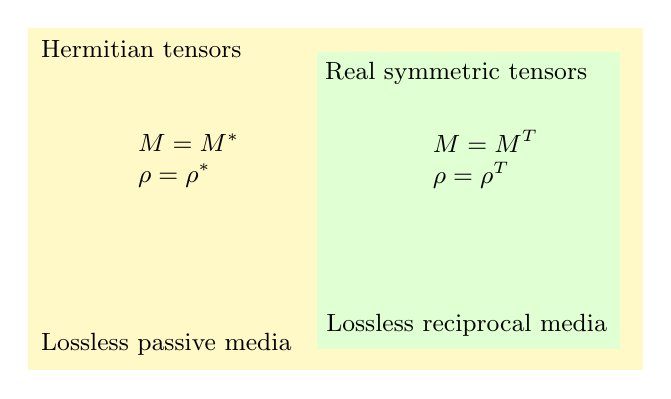
\begin{tikzpicture}[x=0.75pt,y=0.75pt,yscale=-1,xscale=1]
%uncomment if require: \path (0,174); %set diagram left start at 0, and has height of 174

%Shape: Rectangle [id:dp17906036618777477] 
\draw  [draw opacity=0][fill={rgb, 255:red, 255; green, 248; blue, 199 }  ,fill opacity=1 ] (178,4.33) -- (474,4.33) -- (474,168.9) -- (178,168.9) -- cycle ;
%Shape: Rectangle [id:dp15652548189864945] 
\draw  [draw opacity=0][fill={rgb, 255:red, 224; green, 255; blue, 210 }  ,fill opacity=1 ] (317,15.57) -- (463,15.57) -- (463,158.89) -- (317,158.89) -- cycle ;

% Text Node
\draw (183,9) node [anchor=north west][inner sep=0.75pt]  [font=\small] [align=left] {{\small Hermitian tensors}};
% Text Node
\draw (183,150) node [anchor=north west][inner sep=0.75pt]  [font=\small] [align=left] {{\small Lossless passive media}};
% Text Node
\draw (223,52.4) node [anchor=north west][inner sep=0.75pt]  [font=\small]  {$ \begin{array}{l}
M =M^{*}\\
\rho =\rho ^{*}
\end{array}$};
% Text Node
\draw (319.83,19.49) node [anchor=north west][inner sep=0.75pt]  [font=\small] [align=left] {{\small Real symmetric tensors}};
% Text Node
\draw (320.37,140.99) node [anchor=north west][inner sep=0.75pt]  [font=\small] [align=left] {{\small Lossless reciprocal media}};
% Text Node
\draw (365,52.4) node [anchor=north west][inner sep=0.75pt]  [font=\small]  {$ \begin{array}{l}
M =M^{T}\\
\rho =\rho ^{T}
\end{array}$};


\end{tikzpicture}


\section*{Example of citations}
Reference~\cite{pierce2019acoustics} is a good book \cite{blackstock2000fundamentals}.

\begin{figure}
\centering\includegraphics[width=0.3\linewidth]{fig/test}\caption{Figure generated by MATLAB. If you zoom in, you will see that the entire graphic is vectorized. Nice!}
\end{figure}


\printbibliography[heading=bibintoc, title={References}]
\end{document}